% arara: xelatex
%% arara: xelatex


% https://koalatea.io/r-knn-regression/
% http://freerangestats.info/blog/2017/04/09/propensity-v-regression
% https://economics.stackexchange.com/questions/45335/what-is-the-difference-between-ate-and-att
% https://kosukeimai.github.io/MatchIt/articles/matching-methods.html


\documentclass[14pt,xcolor=dvipsnames,handout]{beamer}


% !TEX root = om_metrics_14.tex

%\usepackage{epsdice} % dice 1-6 for probability :)

% \usepackage[absolute,overlay]{textpos}

% \usefonttheme[onlymath]{serif}

\usefonttheme{professionalfonts}
% by default beamer changes math fonts for better visibility for projection
% this professionalfonst theme removes this behavior


\usepackage[orientation=portrait,size=custom,width=25.4,height=19.05]{beamerposter}




%25,4 см 19,05 см размеры слайда в powerpoint

\usetheme{metropolis}
\metroset{
  %progressbar=none,
  numbering=none,
  subsectionpage=progressbar,
  block=fill
}

%\usecolortheme{seahorse}

\usepackage{xunicode} % хак для акцентов!
% https://tex.stackexchange.com/questions/28003/

\usepackage{fontspec}
\usepackage{polyglossia}
\setmainlanguage{russian}


% \usepackage{fontawesome5} % removed [fixed]
\setmainfont[Ligatures=TeX]{Myriad Pro}
% \setsansfont{Myriad Pro}




% why do we need \newfontfamily:
% http://tex.stackexchange.com/questions/91507/
\newfontfamily{\cyrillicfonttt}{Myriad Pro}
\newfontfamily{\cyrillicfont}{Myriad Pro}
%\newfontfamily{\cyrillicfontbs}{Myriad Pro}
\newfontfamily{\cyrillicfontsf}{Myriad Pro}


% https://tex.stackexchange.com/questions/175860/why-does-unicode-math-break-the-kerning-of-accents-in-combination-with-amssymb
% "You shouldn't be using amssymb together with unicode-math"
\usepackage{amsmath}
\usepackage{amsthm} % amssymb 


% https://tex.stackexchange.com/questions/483722/
% \usepackage[MnSymbol]{mathspec}  % Includes amsmath.
% \usepackage{mathspec}  % Includes amsmath.
% \setmathsfont(Digits,Latin,Greek,Symbols)[Numbers={Lining,Proportional}]{Latin Modern Math}
% mathspec must be loaded earlier than amsmath



%\usepackage{bm}

% \usepackage{fdsymbol} % \nperp

% \usepackage{unicode-math} % \symbf
% \setmathfont{Latin Modern Math}



\usepackage{centernot}

\usepackage{graphicx}

\usepackage{wrapfig}
% \usepackage{animate} % animations :)
% \usepackage{tikz}
%\usetikzlibrary{shapes.geometric,patterns,positioning,matrix,calc,arrows,shapes,fit,decorations,decorations.pathmorphing}
% \usepackage{pifont}
\usepackage{comment}
\usepackage[font=small,labelfont=bf]{caption}
\captionsetup[figure]{labelformat=empty}
% \includecomment{techno}



%Расположение

\setbeamersize{text margin left=15 mm,text margin right=5mm} 
\setlength{\leftmargini}{38 pt}

%\usepackage{showframe}
%\usepackage{enumitem}
% \setlist{leftmargin=5.5mm}


%Цвета от дирекции

\definecolor{dirblack}{RGB}{58, 58, 58}
\definecolor{dirwhite}{RGB}{245, 245, 245}
\definecolor{dirred}{RGB}{149, 55, 53}
\definecolor{dirblue}{RGB}{0, 90, 171}
\definecolor{dirorange}{RGB}{235, 143, 76}
\definecolor{dirlightblue}{RGB}{75, 172, 198}
\definecolor{dirgreen}{RGB}{155, 187, 89}
\definecolor{dircomment}{RGB}{128, 100, 162}

\setbeamercolor{title separator}{bg=dirlightblue!50, fg=dirblue}

%Цвета блоков

% Голубой блок!
\setbeamercolor{block title}{bg=dirblue!30,fg=dirblack}
\setbeamercolor{block title example}{bg=dirlightblue!50,fg=dirblack}
\setbeamercolor{block body example}{bg=dirlightblue!20,fg=dirblack}

\AtBeginEnvironment{exampleblock}{\setbeamercolor{itemize item}{fg=dirblack}}
%\setbeamertemplate{blocks}[rounded][shadow]

% Набор команд для удобства верстки

% Набор команд для структуризации

%\newcommand{\quest}{\faQuestionCircleO}
%\faPencilSquareO \faPuzzlePiece \faQuestionCircleO  \faIcon*[regular]{file} {\textcolor{dirblue}
%\newcommand{\quest}{\textcolor{dirblue}{\boxed{\textbf{?}}}
%\newcommand{\task}{\faIcon{tasks}}
%\newcommand{\exmpl}{\faPuzzlePiece}
%\newcommand{\dfn}{\faIcon{pen-square}}
%\newcommand{\quest}{\textcolor{dirblue}{\faQuestionCircle[regular]}}
%\newcommand{\acc}[1]{\textcolor{dirred}{#1}}
%\newcommand{\accm}[1]{\textcolor{dirred}{#1}}
%\newcommand{\acct}[1]{\textcolor{dirblue}{#1}}
%\newcommand{\acctm}[1]{\textcolor{dirblue}{#1}}
%\newcommand{\accex}[1]{\textcolor{dirblack}{\bf #1}}
%\newcommand{\accexm}[1]{\textcolor{dirblack}{ \mathbf{#1}}}
%\newcommand{\acclp}[1]{\textcolor{dirorange}{\it #1}}
\newcommand{\todo}[1]{\textcolor{dircomment}{\bf #1}}
%\newcommand{\graylink}[1]{{\fontsize{11}{12}\selectfont \textcolor{gray}{#1}}}
%\newcommand{\figcaption}[1]{{\fontsize{18}{20}\selectfont #1}}


\newcommand{\videotitle}[1]{
    {\fontsize{33}{30}\selectfont \textcolor{dirblue}{\textbf{#1}} }

    %\todo{название видеофрагмента}
}

\newcommand{\lecturetitle}[1]{
  {\fontsize{33}{30}\selectfont \textcolor{dirblue}{\textbf{#1}} }

    %\todo{название лекции}
}





%\newcommand{\spcbig}{\vspace{-10 pt}}
%\newcommand{\spcsmall}{\vspace{-5 pt}}

%\usepackage{listings}
%\lstset{
%xleftmargin=0 pt,
%  basicstyle=\small, 
%  language=Python,
  %tabsize = 2,
%  backgroundcolor=\color{mc!20!white}
%}



%\newcommand{\mypart}[1]{\begin{frame}[standout]{\huge #1}\end{frame}}

\setbeamercolor{background canvas}{bg=}

% frame title setup
\setbeamercolor{frametitle}{bg=,fg=dirblue}
\setbeamertemplate{frametitle}[default][left]

\addtobeamertemplate{frametitle}{\hspace*{0.1 cm}}{\vspace*{0.25cm}}


%Шрифты
\setbeamerfont{frametitle}{family=\rmfamily,series=\bfseries,size={\fontsize{33}{30}}}
\setbeamerfont{framesubtitle}{family=\rmfamily,series=\bfseries,size={\fontsize{26}{20}}}


% удобнее знать номер слайда, чтобы вносить правки!  

\setbeamercolor{footline}{fg=dircomment}
\setbeamerfont{footline}{series=\bfseries, size={\fontsize{12}{14}}}
%\setbeamertemplate{footline}[page number]


\defbeamertemplate{footline}{custom footline}
{%
  \hspace*{\fill}%
  \usebeamercolor[fg]{page number in head/foot}%
  \usebeamerfont{page number in head/foot}%
  page: \insertpagenumber\,/\,\insertpresentationendpage%
  \hspace{20pt}%
  slide: \insertframenumber\,/\,\inserttotalframenumber%
  %\hspace*{\fill}
  \vskip2pt%
}
%\setbeamertemplate{footline}[custom footline]

\usepackage{physics}



% tikz block

\usepackage{pgfplots}
\pgfplotsset{compat=newest}

\usepackage{tikz}
\usetikzlibrary{calc}
\usetikzlibrary{quotes,angles}
\usetikzlibrary{arrows}
\usetikzlibrary{arrows.meta}
\usetikzlibrary{positioning,intersections,decorations.markings}
\usetikzlibrary{patterns}

\usepackage{tkz-euclide} 
%\tikzset{>=latex}

\tikzset{cross/.style={cross out, draw=black, minimum size=2*(#1-\pgflinewidth), inner sep=0pt, outer sep=0pt},
%default radius will be 1pt. 
cross/.default={5pt}}

\colorlet{veca}{red}
\colorlet{vecb}{blue}
\colorlet{vecc}{olive}


\newcommand{\grid}{\draw[color=gray,step=1.0,dotted] (-2.1,-2.1) grid (9.6,6.1)}

% end tikz block

\newcommand{\R}{\mathbb{R}}
\newcommand{\Rot}{\mathrm{R}}
\newcommand{\HH}{\mathrm{H}}
\newcommand{\Id}{\mathrm{I}}
\newcommand{\RR}{\mathbb{R}}
\newcommand{\ZZ}{\mathbb{Z}}
\newcommand{\la}{\lambda}
\let\P\relax
\newcommand{\P}{\mathbb{P}}
\newcommand{\E}{\mathbb{E}}

\newcommand{\cN}{\mathcal{N}}
\newcommand{\dN}{\mathcal{N}}

\newcommand{\qL}{q_{\text{left}}}
\newcommand{\qR}{q_{\text{right}}}



\newcommand{\ba}{\mathbf{a}}
\newcommand{\be}{\mathbf{e}}
\newcommand{\bb}{\mathbf{b}}
\newcommand{\bc}{\mathbf{c}}
\newcommand{\bd}{\mathbf{d}}
\newcommand{\bx}{\mathbf{x}}
\newcommand{\bff}{\mathbf{f}} % \bf is already def
\newcommand{\bv}{\mathbf{v}}
\newcommand{\bzero}{\mathbf{0}}



\DeclareMathOperator{\Var}{Var}
\DeclareMathOperator{\sVar}{sVar}
\DeclareMathOperator{\Cov}{Cov}
\DeclareMathOperator{\sCov}{sCov}
\DeclareMathOperator{\sCorr}{sCorr}
\DeclareMathOperator{\Corr}{Corr}
\DeclareMathOperator{\Med}{Med}


\DeclareMathOperator{\plim}{plim}
\DeclareMathOperator{\sign}{sign}


\newcommand{\graylink}[1]{{\fontsize{11}{12}\selectfont \textcolor{gray}{#1}}}
\newcommand{\figcaption}[1]{{\fontsize{18}{20}\selectfont #1}}





\begin{document}


\begin{frame} % название лекции


\lecturetitle{Вариации ETS}

\end{frame}


% !TEX root = ../om_ts_03.tex

\begin{frame} % название фрагмента

\videotitle{Модель ETS: дампированный тренд}

\end{frame}



\begin{frame}{Модель ETS: дампированный тренд}
  \begin{itemize}[<+->]
    \item Идея дампированного тренда. 
    \item Новый коэффициент в модели. 
    \item Формулы для прогнозов.
  \end{itemize}

\end{frame}

\begin{frame}{Проблема тренда в ETS(AAN)}

  В ETS(AAN) модели \alert{скорость роста} тренда $\ell_t$ определена формулой
  \[
  b_t = b_{t-1} + \beta u_t, \text{ стартовое } b_0.
  \]
  \pause
  Следовательно,
  \[
  \E(b_t) = \E(b_{t-1}), \quad \E(b_{T+h} \mid b_T) = b_T.
  \]
  \pause
  Долгосрочный прогноз положительного показателя при $b_T < 0$ 
  станет отрицательным. 
\end{frame}

\begin{frame}{Противоречие}
  Краткосрочные ожидания изменения показателя. 

  \alert{Хотим тренд} в модели. 

  \pause
  Долгосрочная невозможность отрицательных значений. 

  \alert{Не хотим тренд} в модели.

  \pause
  Решение: \alert{дампированный} или \alert{затухающий} тренд. 
\end{frame}

\begin{frame}{Лишние параметры — дорого!}
  Хотим более богатую динамику тренда — нужны \alert{дополнительные} параметры. 

  \pause
  Дополнительные параметры — риск \alert{переподгонки} модели, 
  более \alert{широкие доверительные интервалы} для оставшихся параметров. 

  \pause 
  Обойдёмся всего \alert{одним} новым параметром!
\end{frame}

\begin{frame}
  \frametitle{Дампированный тренд}

  Вводим параметр затухания тренда $\phi \in (0; 1)$ в уравнение наклона:
  \[
  b_t = \phi b_{t-1} + \beta u_t, \text{ стартовое } b_0.
  \]
  \pause
  И в остальные уравнения:
  \[
    \begin{cases}
      y_t = \ell_{t-1} + \phi b_{t-1} + u_t; \\
     \ell_t = \ell_{t-1} + \phi b_{t-1} + \alpha u_t, \text{ стартовое } \ell_0; \\
    \end{cases}
  \]

\end{frame}


\begin{frame}{Общий вид ETS(AAdN)}

  \[
    \begin{cases}
      y_t = \ell_{t-1} + \phi b_{t-1} + u_t; \\
     \ell_t = \ell_{t-1} + \phi b_{t-1} + \alpha u_t, \text{ стартовое } \ell_0; \\
     b_t = \phi b_{t-1} + \beta u_t, \text{ стартовое } b_0; \\
     u_t \sim \dN(0;\sigma^2) \text{ и независимы.} \\
    \end{cases}
  \]
  \pause

  Параметры (\alert{6 штук}): $\alpha$, $\sigma^2$, $\ell_0$, $b_0$, $\beta$, $\phi$. 
\end{frame}

\begin{frame}
  \frametitle{ETS(AAdN): прогнозируем}

  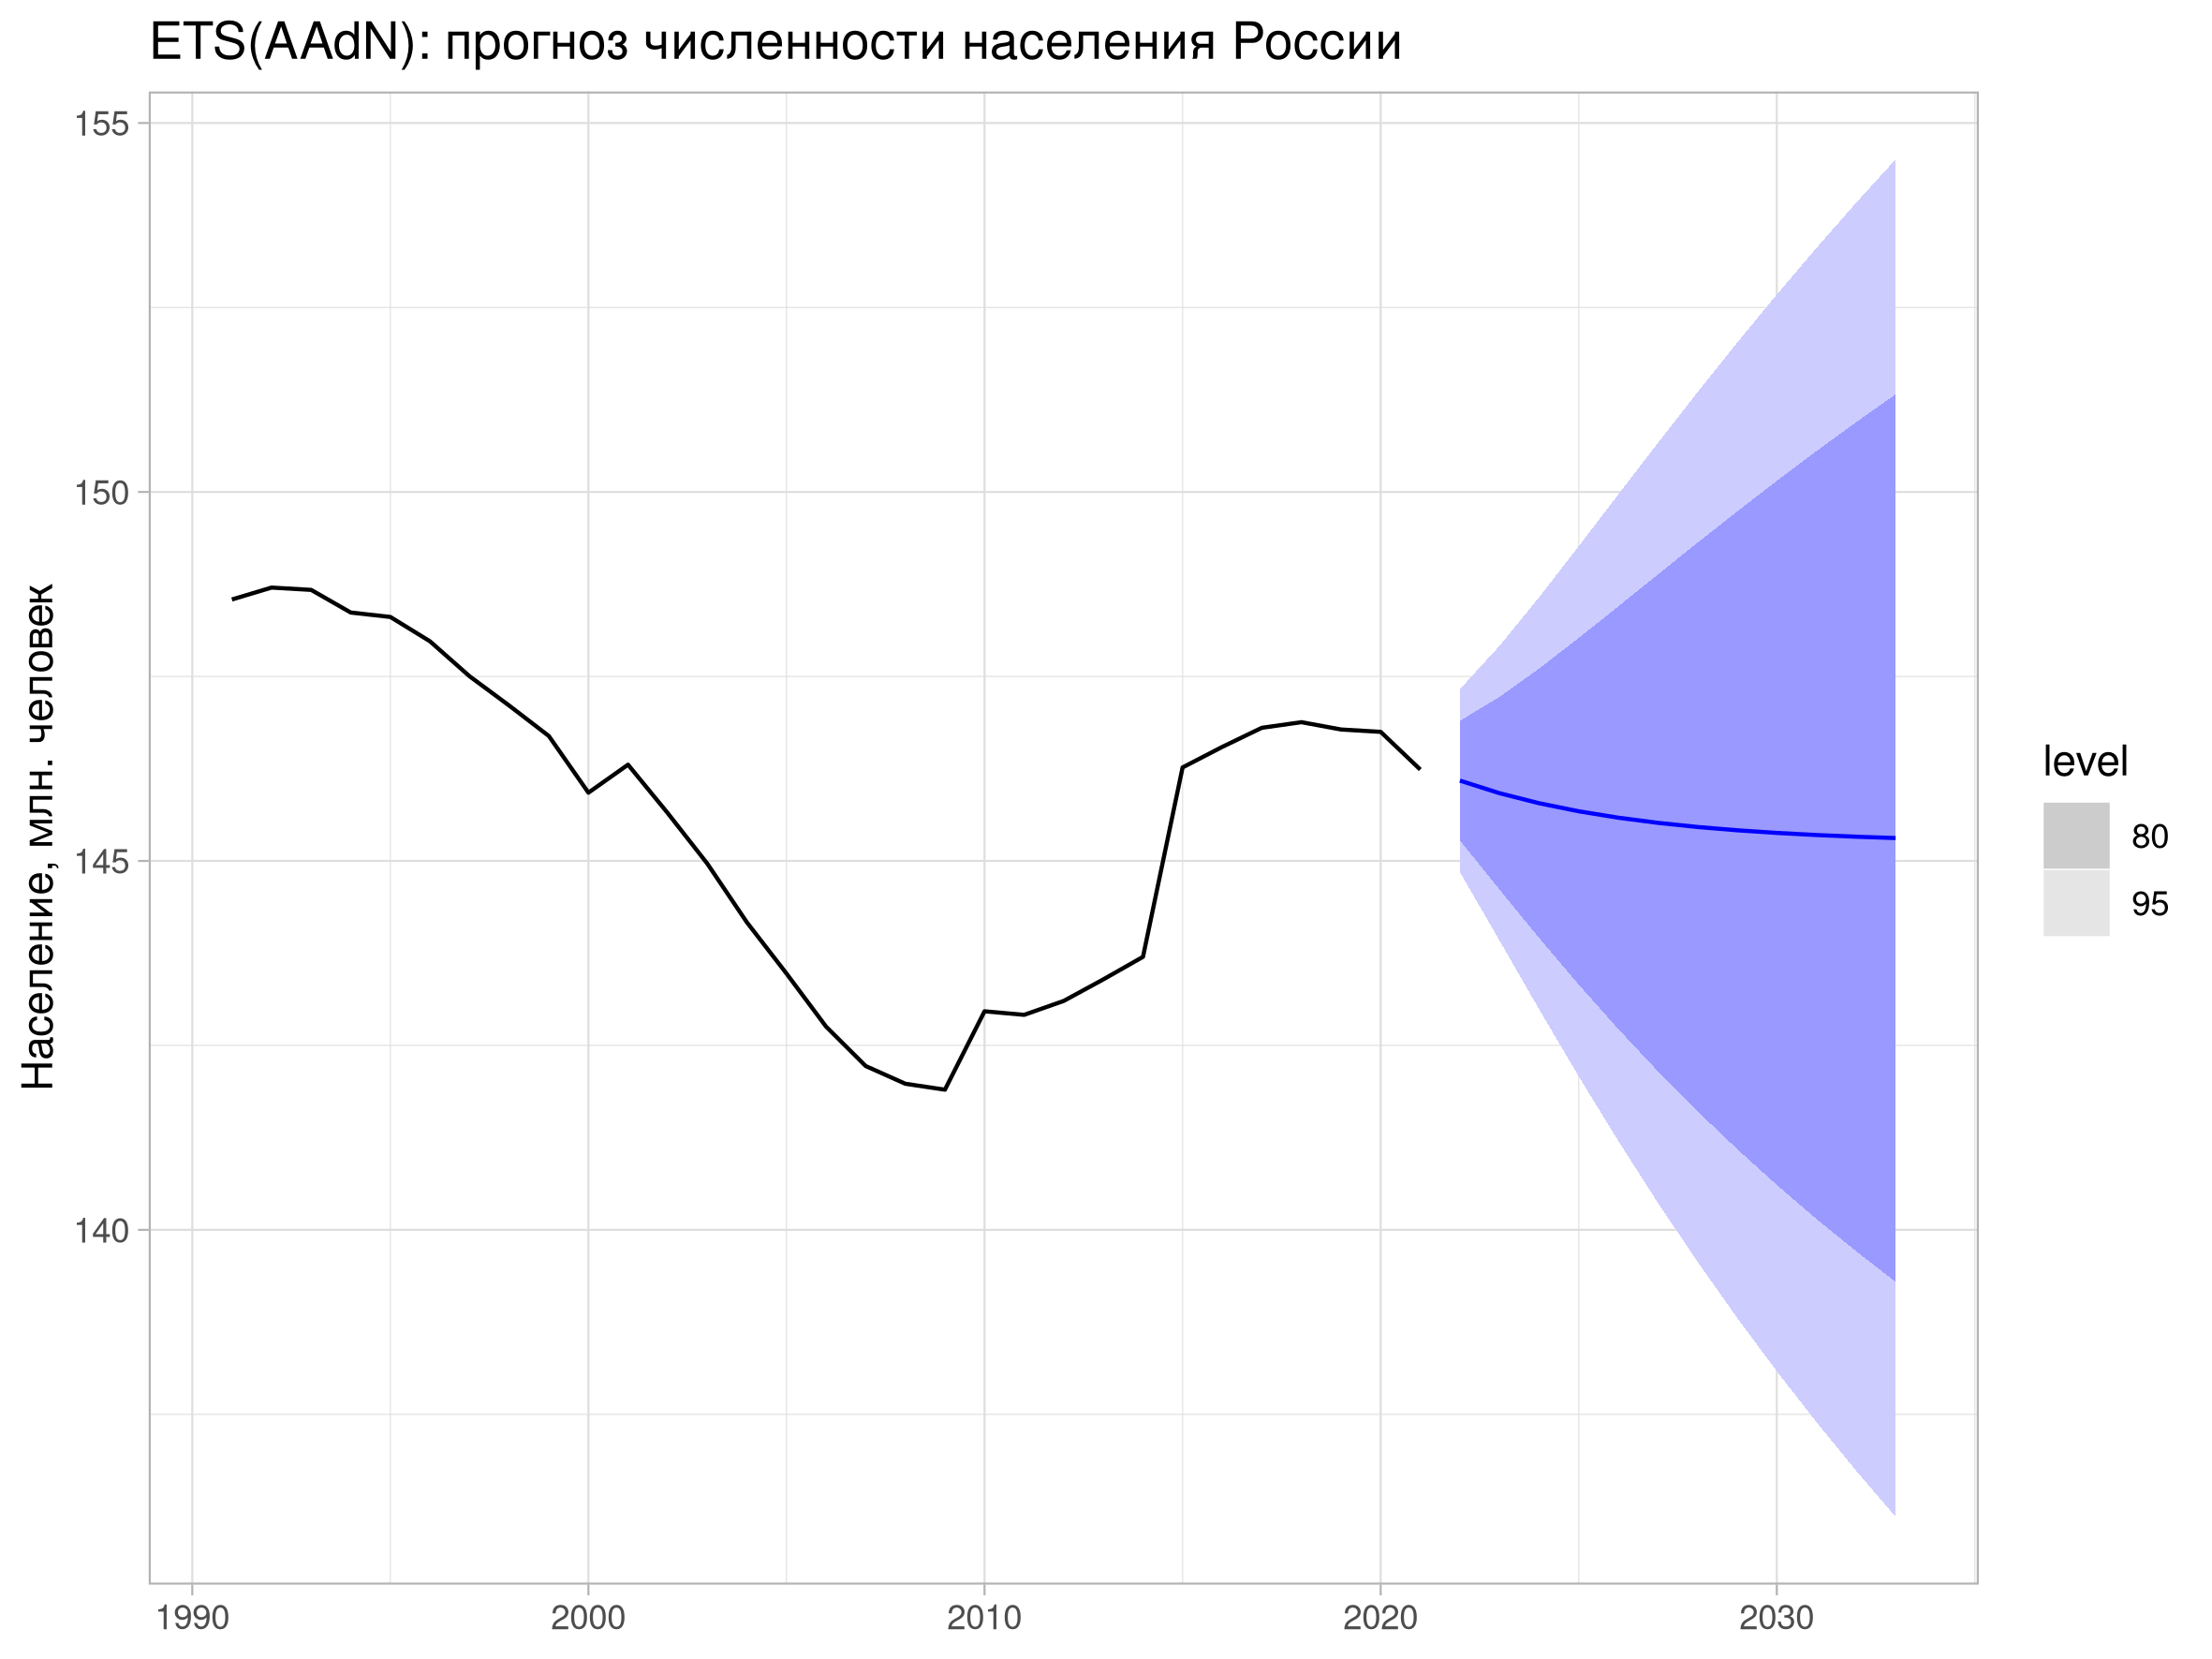
\includegraphics[width=\textwidth]{pictures/om_ts_03-019.png}
  
  % https://www.youtube.com/watch?v=e5WxxvjR9c4
  % я никак не пойму в чём секрет, тренд если есть, то его сразу нет. 

\end{frame}


\begin{frame}
  \frametitle{Прогноз на 1 шаг вперёд}

  \[
      \begin{cases}
        y_t = \ell_{t-1} + \phi b_{t-1} + u_t; \\
       \ell_t = \ell_{t-1} + \phi b_{t-1} + \alpha u_t, \text{ стартовое } \ell_0; \\
       b_t = \phi b_{t-1} + \beta u_t, \text{ стартовое } b_0; \\
       u_t \sim \dN(0;\sigma^2) \text{ и независимы.} \\
       \end{cases}
  \]
  \pause
\[
y_{T+1} = \ell_T + \phi b_T + u_{T+1}  
\]
\pause
\[
  (y_{T+1} \mid \mathcal F_T) \sim \dN(\ell_T + \phi b_T; \sigma^2)  
\]

\end{frame}


\begin{frame}
  \frametitle{Прогноз на 2 шага вперёд}

  \[
    \begin{cases}
      y_t = \ell_{t-1} + \phi b_{t-1} + u_t; \\
     \ell_t = \ell_{t-1} + \phi b_{t-1} + \alpha u_t, \text{ стартовое } \ell_0; \\
     b_t = \phi b_{t-1} + \beta u_t, \text{ стартовое } b_0; \\
     u_t \sim \dN(0;\sigma^2) \text{ и независимы.} \\
     \end{cases}
   \]
  \pause
  \begin{multline*}
    y_{T+2} = \ell_{T+1} + \phi b_{T+1} + u_{T+2} = (\ell_T + \phi b_T + \alpha u_{T+1}) +\\
    + \phi(\phi b_T + \beta u_{T+1}) + u_{T+2} 
  \end{multline*}
   \pause
  \[
  (y_{T+2} \mid \mathcal F_T) \sim \dN(\ell_T + (\phi + \phi^2) b_T; \sigma^2((\alpha + \phi \beta)^2 + 1))
  \]
  
\end{frame}



\begin{frame}{ETS(AAdN): итоги}

  \begin{itemize}[<+->]
    \item На малом горизонте прогнозирования \alert{тренд есть}. 
    \item На большом горизонте прогнозирования \alert{тренда нет}.  
    \item \alert{Один} дополнительный параметр. 
    \item Можно получить ETS(AAdA) модель \alert{с сезонностью}. 
  \end{itemize}
\end{frame}



% !TEX root = ../om_ts_03.tex

\begin{frame} % название фрагмента

\videotitle{ETS: мультипликативные компоненты}

\end{frame}



\begin{frame}{ETS: мультипликативные компоненты}
  \begin{itemize}[<+->]
    \item Мультипликативные составляющие.
    \item Формулы для прогнозов.
  \end{itemize}

\end{frame}


\begin{frame}
  \frametitle{Разная амплитуда колебаний}

  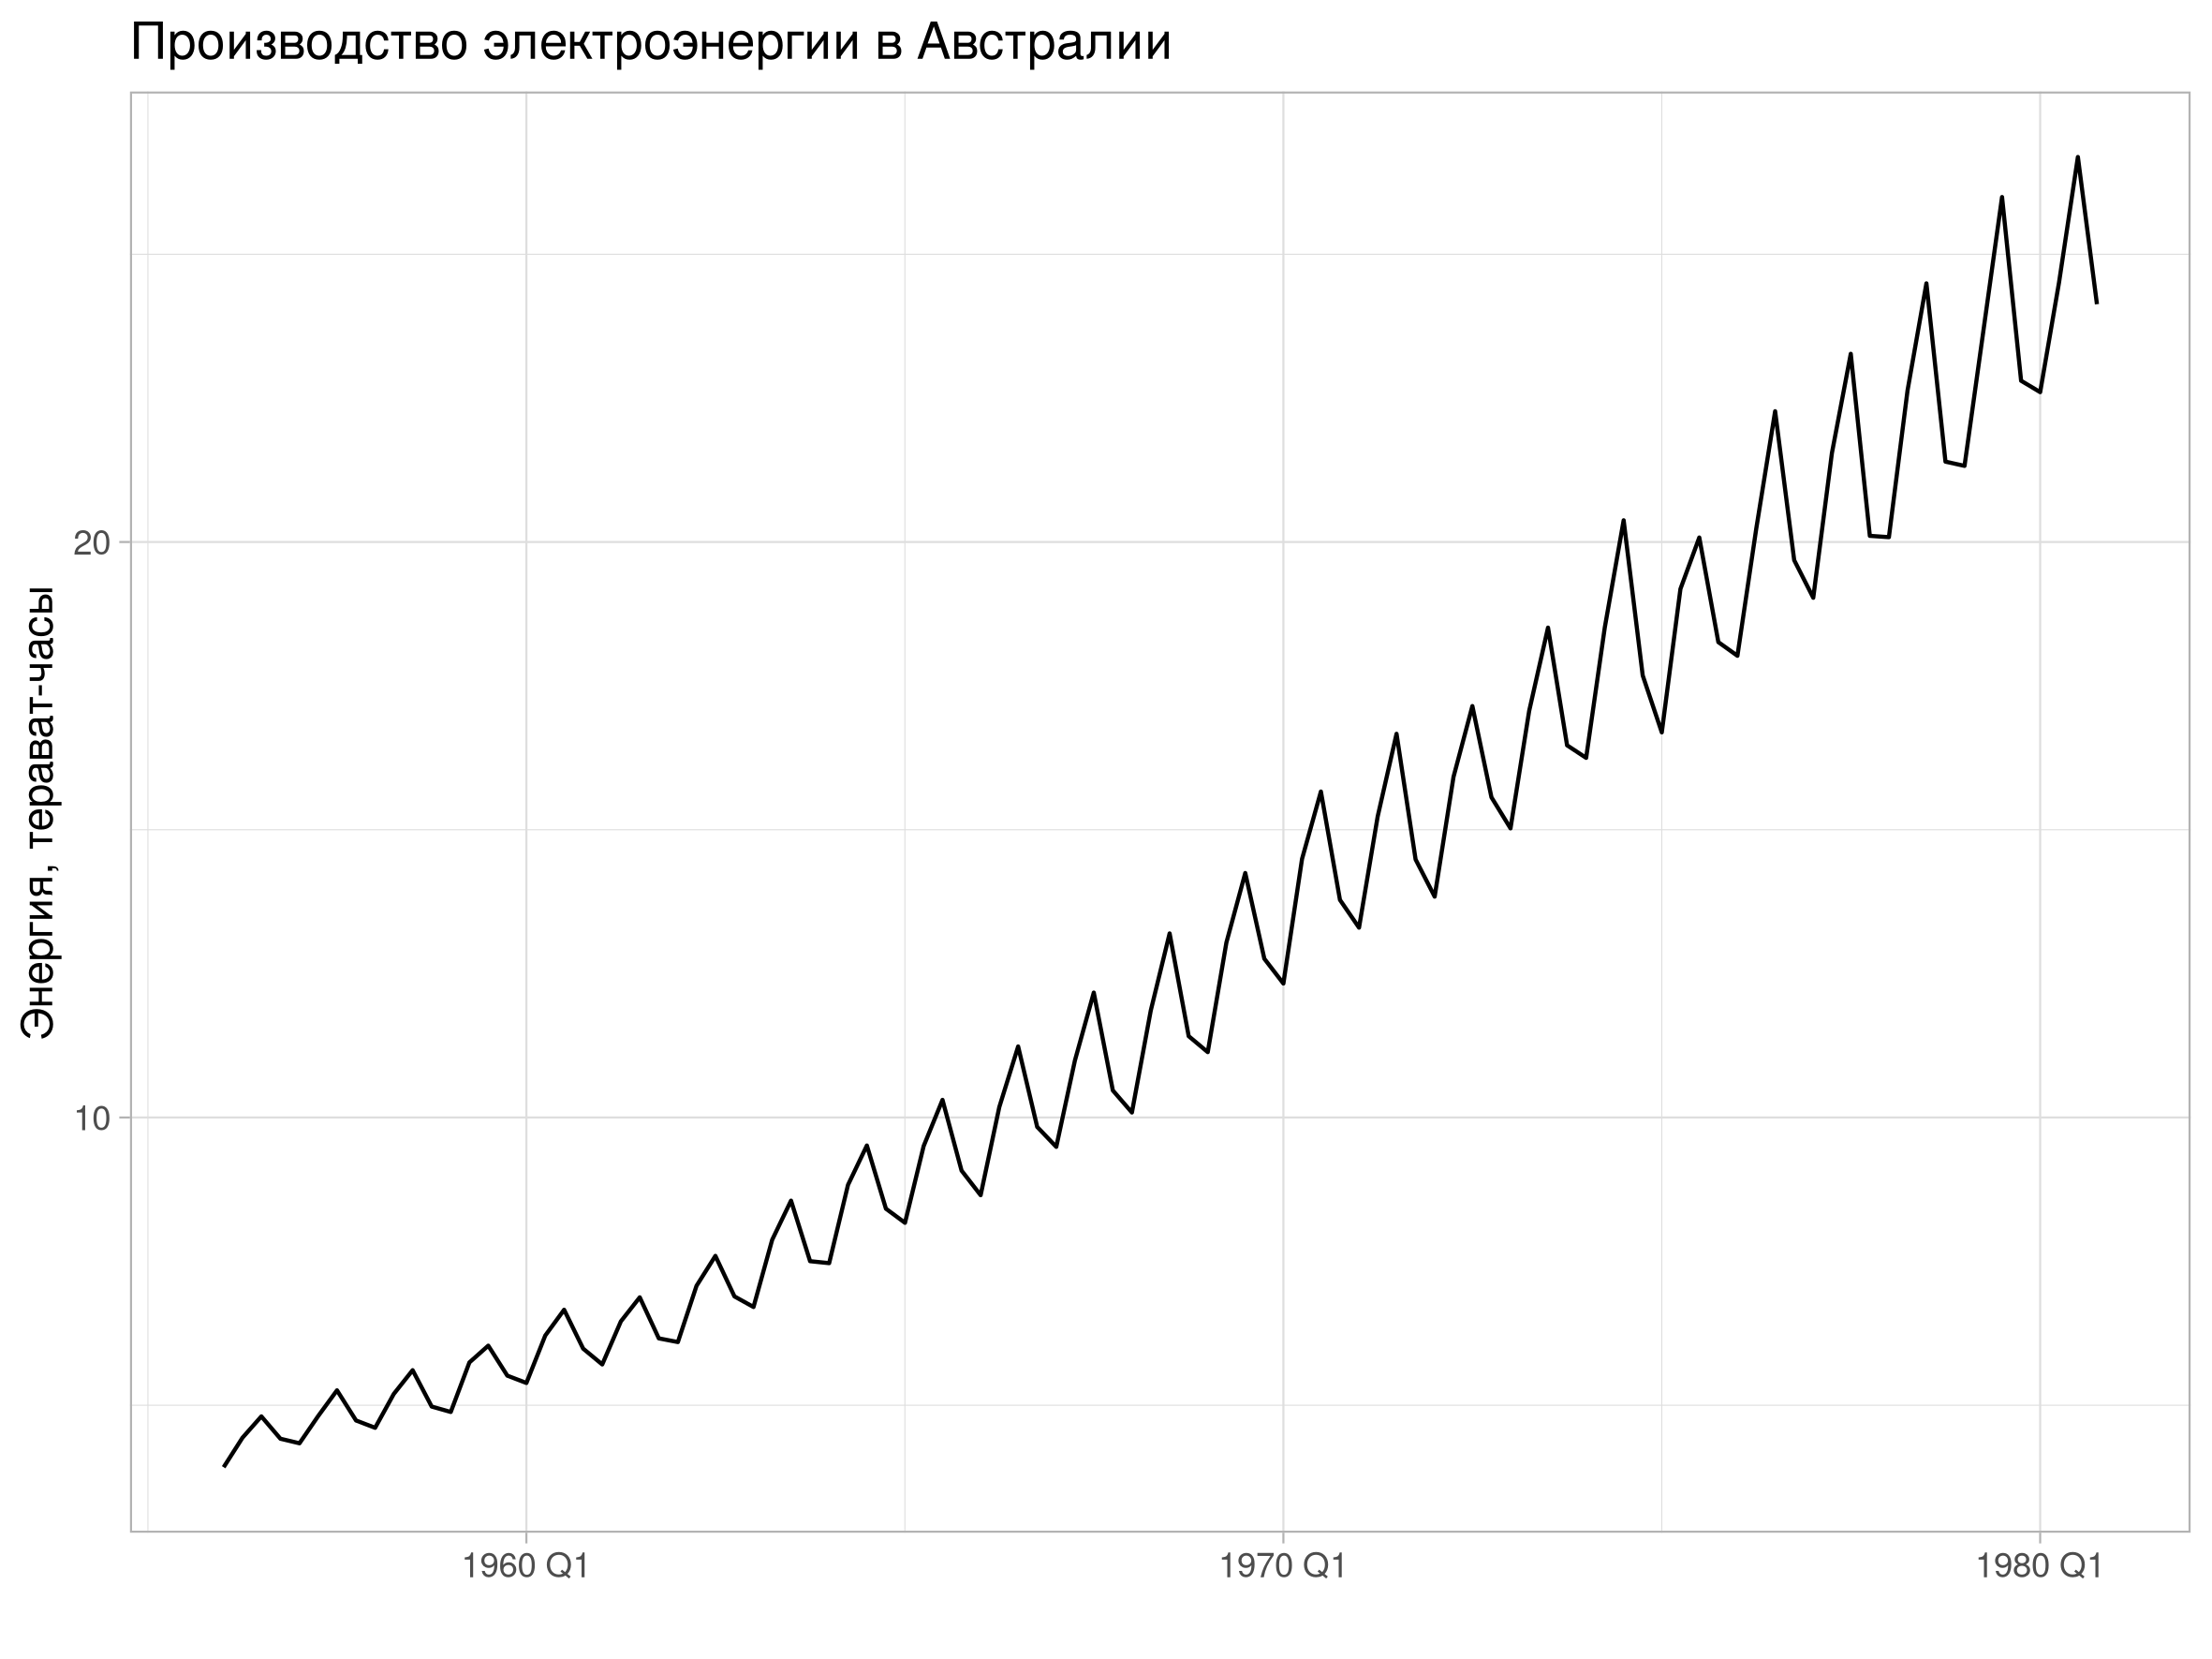
\includegraphics[width=\textwidth]{pictures/om_ts_03-033.png}

\end{frame}


\begin{frame}  
  \frametitle{Разная амплитуда колебаний}

  Возможные \alert{решения}:
  \begin{itemize}[<+->]
    \item Переход к логарифмам, $y_t \to \ln y_t$.
    \item Преобразование Бокса-Кокса, $y_t \to bc(y_t, \lambda)$.
    \item Мультипликативные компоненты. 
  \end{itemize}

\end{frame}



\begin{frame}
  \frametitle{ETS(MNM): уравнения}

  ETS(MNM) для месячных данных:
  
  \[
    \begin{cases}
     y_t = \ell_{t-1} \cdot s_{t-12} \cdot (1 + u_t); \\
    \ell_t = \ell_{t-1}\cdot  (1 + \alpha u_t), \text{ стартовое } \ell_0; \\
    s_t = s_{t-12}\cdot (1 + \gamma u_t), \text{ стартовые } s_0, \ldots, s_{-11}; \\
    u_t \sim \dN(0;\sigma^2) \text{ и независимы.} \\
    \end{cases}
  \]

  \pause
  ETS(ANA):
  \[
    \begin{cases}
     y_t = \ell_{t-1} + s_{t-12} + u_t; \\
    \ell_t = \ell_{t-1} + \alpha u_t, \text{ стартовое } \ell_0; \\
    s_t = s_{t-12} + \gamma u_t, \text{ стартовые } s_0, \ldots, s_{-11}; \\
    \end{cases}
  \]

\end{frame}



\begin{frame}
  \frametitle{ETS(MNM): параметры}

  ETS(MNM) для месячных данных:
  
  \[
    \begin{cases}
     y_t = \ell_{t-1} \cdot s_{t-12} \cdot (1 + u_t); \\
    \ell_t = \ell_{t-1}\cdot  (1 + \alpha u_t), \text{ стартовое } \ell_0; \\
    s_t = s_{t-12}\cdot (1 + \gamma u_t), \text{ стартовые } s_0, \ldots, s_{-11}; \\
    u_t \sim \dN(0;\sigma^2) \text{ и независимы.} \\
    \end{cases}
  \]

\pause
\alert{Несезонные} параметры: $\alpha$, $\sigma^2$, $\ell_0$.

\pause
\alert{Сезонные} параметры: $\gamma$, $s_0$, $s_{-1}$, \ldots, $s_{-11}$.

\pause
\alert{Ограничение}: $s_0 \cdot s_{-1} \cdot \ldots \cdot s_{-11} = 1$.

\pause
Всего: 15 параметров. 

\end{frame}

\begin{frame}
  \frametitle{Единицы измерения}

  Ряды $y_t$, $\ell_t$  — \alert{исходные} единицы измерения. 

  \pause

  Ряды $s_t$, $u_t$ — доли. 

  \pause

  Ряд $s_t$ измеряется относительно единицы, например, $s_t = 0.9$ — ниже тренда на 10\%.

  Ряд $u_t$ измеряется относительно нуля, например, $u_t = -0.1$ — падение на 10\%.

\end{frame}



\begin{frame}
  \frametitle{ETS(MNM): прогнозируем}

  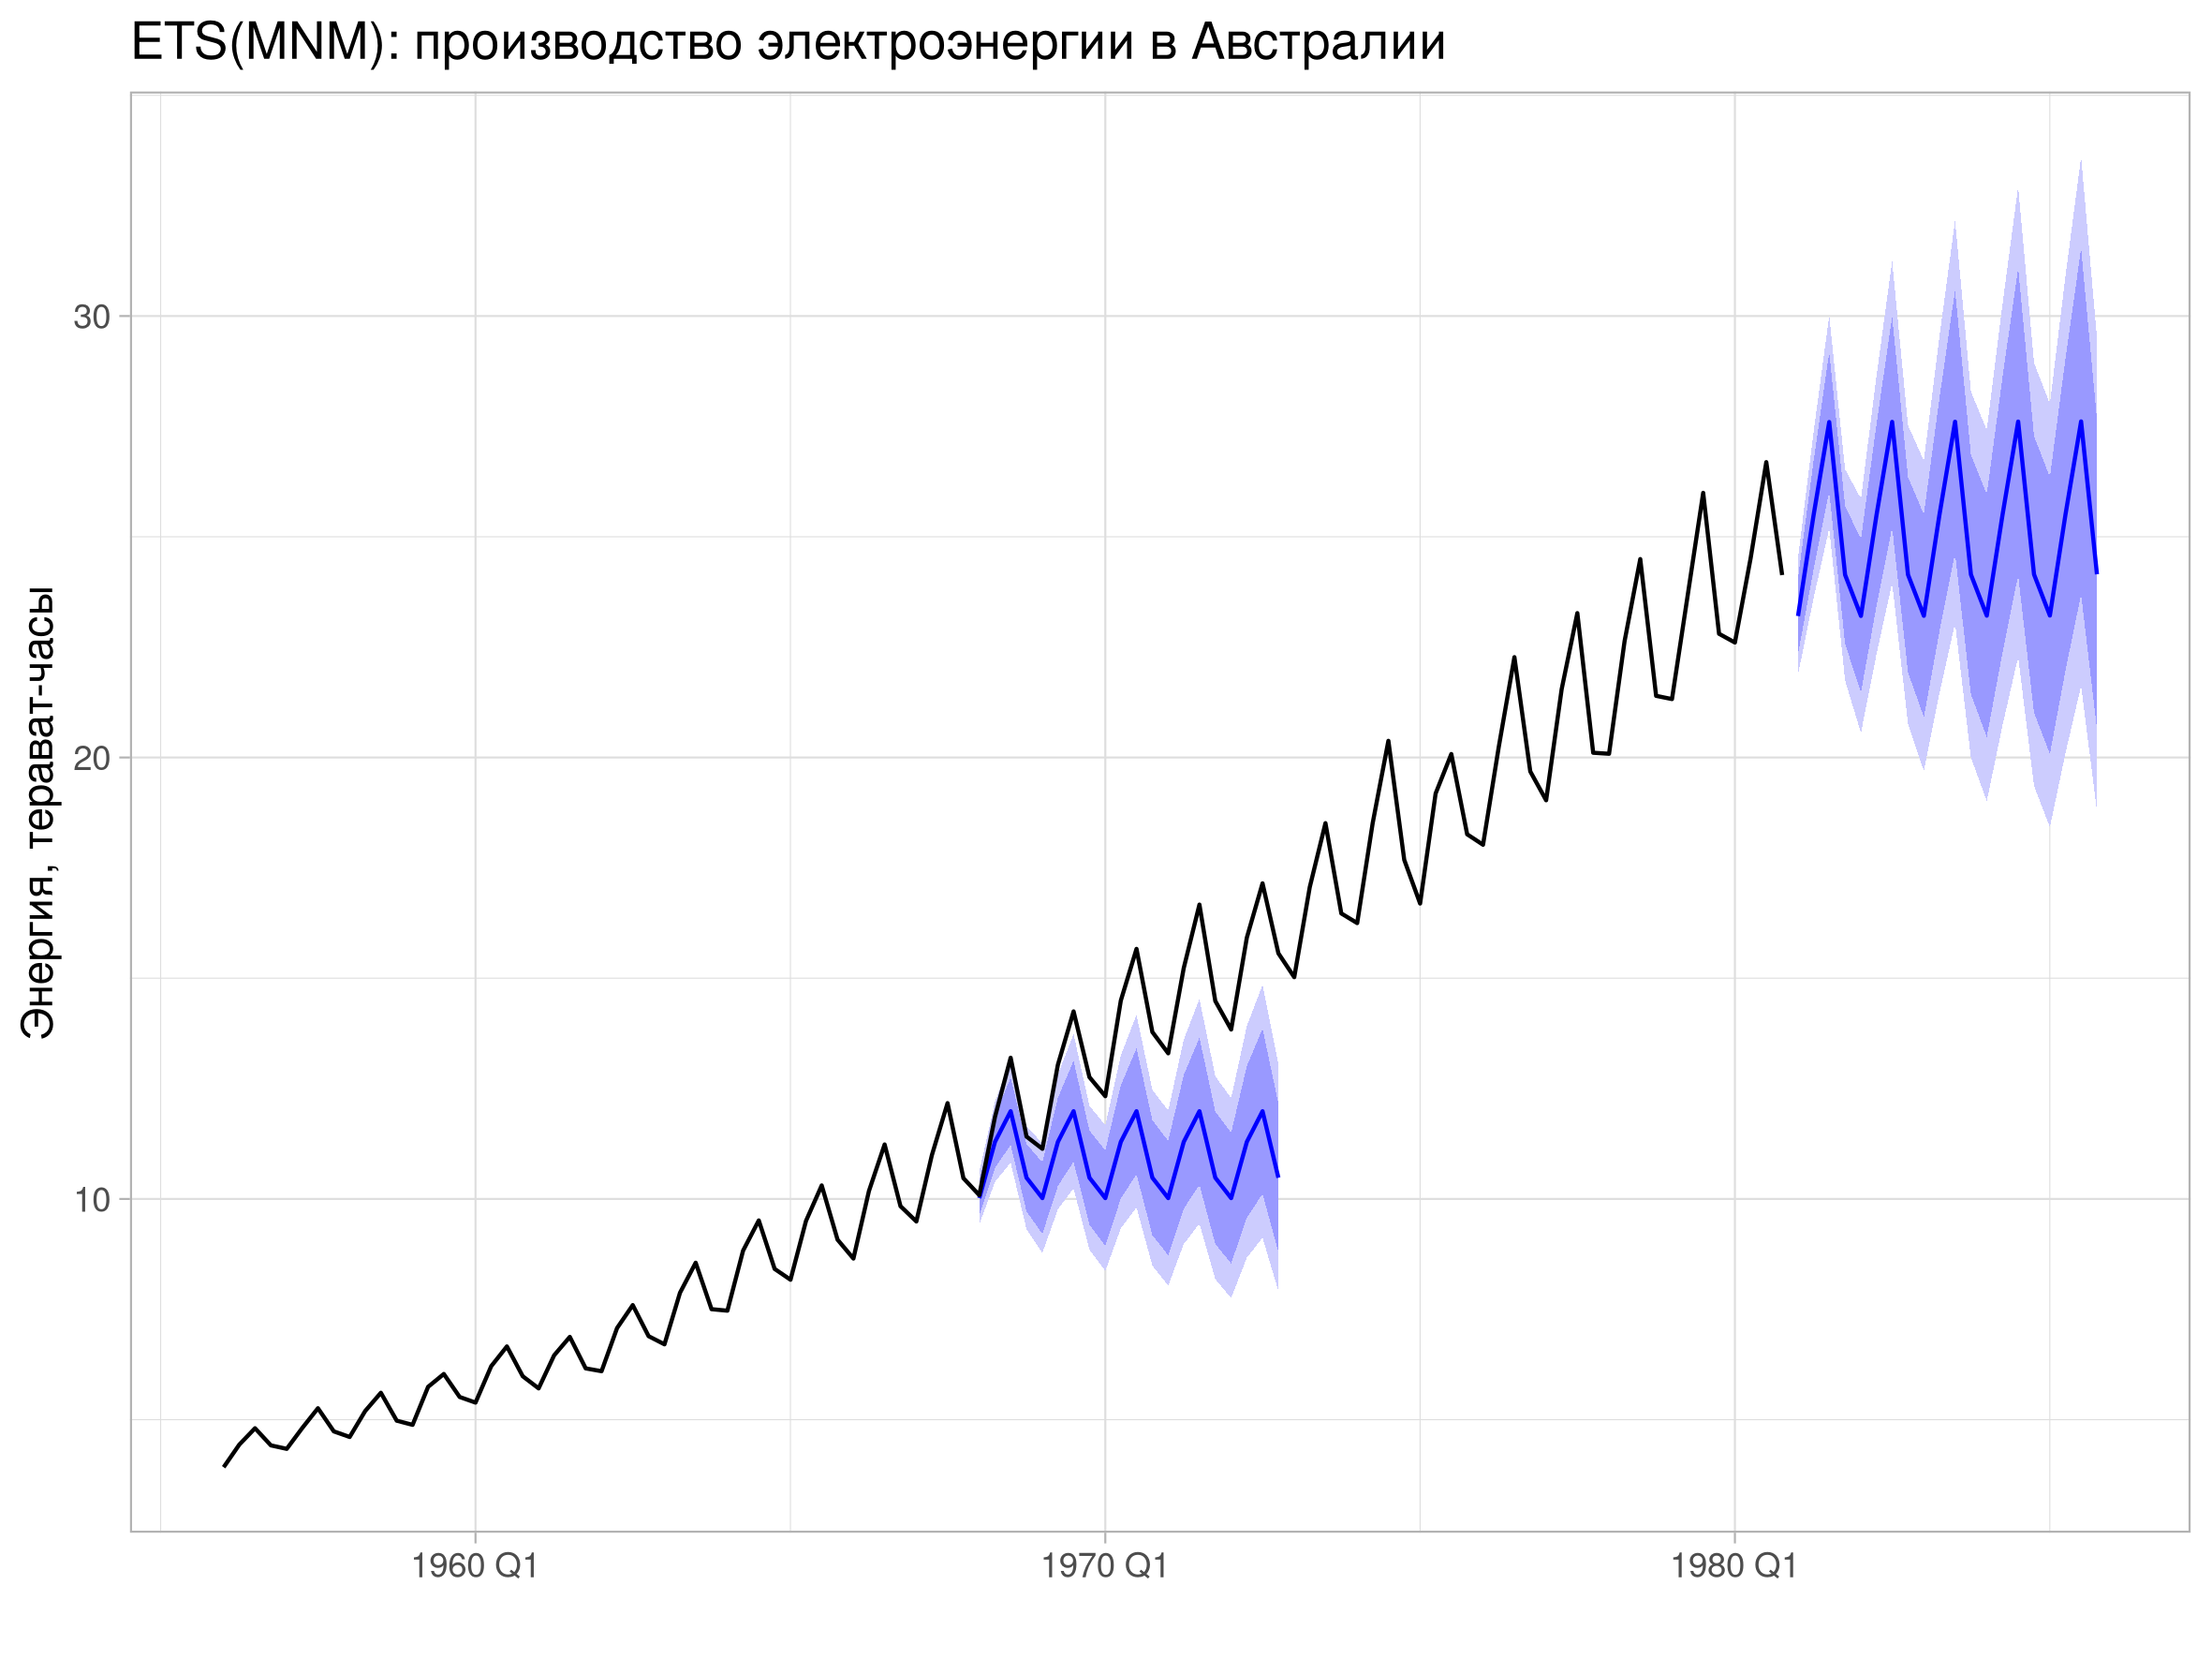
\includegraphics[width=\textwidth]{pictures/om_ts_03-047.png}


\end{frame}


\begin{frame}
  \frametitle{Прогноз на 1 шаг вперёд}

  \[
    \begin{cases}
     y_t = \ell_{t-1} \cdot s_{t-12} \cdot (1 + u_t); \\
    \ell_t = \ell_{t-1}\cdot  (1 + \alpha u_t), \text{ стартовое } \ell_0; \\
    s_t = s_{t-12}\cdot (1 + \gamma u_t), \text{ стартовые } s_0, \ldots, s_{-11}; \\
    u_t \sim \dN(0;\sigma^2) \text{ и независимы.} \\
    \end{cases}
  \]
  \pause
\[
y_{T+1} = \ell_T \cdot s_{T-11} \cdot (1 + u_{T+1})  
\]
\pause
\[
  (y_{T+1} \mid \mathcal F_T) \sim \dN(\ell_T \cdot s_{T-11} ; (\ell_T \cdot s_{T-11})^2\sigma^2)  
\]

\end{frame}


\begin{frame}
  \frametitle{Прогноз на 2 шага вперёд}

  \[
    \begin{cases}
     y_t = \ell_{t-1} \cdot s_{t-12} \cdot (1 + u_t); \\
    \ell_t = \ell_{t-1}\cdot  (1 + \alpha u_t), \text{ стартовое } \ell_0; \\
    s_t = s_{t-12}\cdot (1 + \gamma u_t), \text{ стартовые } s_0, \ldots, s_{-11}; \\
    u_t \sim \dN(0;\sigma^2) \text{ и независимы.} \\
    \end{cases}
  \]
  \pause
  \begin{multline*}
    y_{T+2} = \ell_{T+1} \cdot s_{T-10} \cdot(1 + u_{T+2}) = \\
    = \ell_T (1 + \alpha u_{T+1})\cdot s_{T-10} \cdot(1 + u_{T+2})
  \end{multline*}
   \pause
 \[
 (y_{T+2} \mid \mathcal F_T) \overset{\cdot}{\sim} \dN(\ell_T \cdot s_{T-10}; \ldots )
 \]
  
\end{frame}



\begin{frame}{Мультипликативная ETS: итоги}

  \begin{itemize}[<+->]
    \item Моделирует \alert{разную} амплитуду колебаний. 
    \item Для \alert{положительных рядов}.
    \item Простор для новых \alert{комбинаций}.
  \end{itemize}
\end{frame}





% !TEX root = ../om_ts_03.tex

\begin{frame} % название фрагмента

\videotitle{Собери свой ETS!}

\end{frame}



\begin{frame}{Собери свой ETS: план}
  \begin{itemize}[<+->]
    \item Собираем ETS(MAdM) модель. 
    \item Прогнозы.
  \end{itemize}

\end{frame}


\begin{frame}
  \frametitle{Разная амплитуда колебаний}

  Картинка с сезонным графиком

\end{frame}


\begin{frame}{Хочу разные компоненты}

Сезонность похожа на \alert{мультипликативную}.

\pause

Мультипликативный тренд означал бы \alert{экспоненциальный} рост.

\pause 

Хочу \alert{аддитивный} затухающий тренд.


\end{frame}


\begin{frame}
  \frametitle{ETS(MAdM): уравнения}

  ETS(MNM) для месячных данных:
  
  \[
    \begin{cases}
     y_t = \ell_{t-1} \cdot s_{t-12} \cdot (1 + u_t); \\
    \ell_t = \ell_{t-1}\cdot  (1 + \alpha u_t), \text{ стартовое } \ell_0; \\
    s_t = s_{t-12}\cdot (1 + \gamma u_t), \text{ стартовые } s_0, \ldots, s_{-11}; \\
    u_t \sim \dN(0;\sigma^2) \text{ и независимы.} \\
    \end{cases}
  \]

  \pause
  Как сюда добавить аддитивный тренд?
  \[
    b_t = \phi b_{t-1} + \beta u_t, \text{ стартовое } b_0.
  \]
\end{frame}


\begin{frame}
  \frametitle{ETS(MAdM): уравнения}

  ETS(MAdM) для месячных данных:
  
  \[
    \begin{cases}
     y_t = (\ell_{t-1} + \alert{\phi  b_{t-1}}) \cdot s_{t-12} \cdot (1 + u_t); \\
    \ell_t = (\ell_{t-1} +  \alert{ \phi  b_{t-1}}) \cdot  (1 + \alpha u_t), \text{ стартовое } \ell_0; \\
    \alert{b_t = } \phi  b_{t-1} + \beta (\ell_{t-1} + \phi  b_{t-1}) u_t, \text{ стартовое } b_0; \\
    s_t = s_{t-12}\cdot (1 + \gamma u_t), \text{ стартовые } s_0, \ldots, s_{-11}; \\
    u_t \sim \dN(0;\sigma^2) \text{ и независимы.} \\
    \end{cases}
  \]

  \pause
  Параметры — \alert{18 штук}.


\end{frame}


\begin{frame}
  \frametitle{ETS(MAdM): прогнозируем}

Картинка с прогнозами на 12 шагов вперед

\end{frame}


\begin{frame}
  \frametitle{Прогноз на 1 шаг вперёд}

  \[
    \begin{cases}
     y_t = (\ell_{t-1} + \alert{\phi  b_{t-1}}) \cdot s_{t-12} \cdot (1 + u_t); \\
    \ell_t = (\ell_{t-1} +  \alert{ \phi  b_{t-1}}) \cdot  (1 + \alpha u_t), \text{ стартовое } \ell_0; \\
    \alert{b_t = } \phi  b_{t-1} + \beta (\ell_{t-1} + \phi  b_{t-1}) u_t, \text{ стартовое } b_0; \\
    s_t = s_{t-12}\cdot (1 + \gamma u_t), \text{ стартовые } s_0, \ldots, s_{-11}; \\
    u_t \sim \dN(0;\sigma^2) \text{ и независимы.} \\
    \end{cases}
  \]
  \pause
\[
y_{T+1} = (\ell_T + \phi b_T)\cdot s_{T-11} \cdot (1 + u_{T+1})  
\]
\pause
\[
  (y_{T+1} \mid \mathcal F_T) \sim \dN((\ell_T + \phi b_T) \cdot s_{T-11} ; (\ell_T + \phi b_T)^2 \cdot s_{T-11}^2\sigma^2)  
\]

\end{frame}




\begin{frame}
  \frametitle{Сколько всего ETS моделей?}

  
  \alert{Ошибка}: A, M.
  
  \alert{Тренд}: N, A, Ad, M, Md. 
  
  \alert{Сезонность}: N, A, M.

  \pause
  A — \alert{аддитивная} составляющая. 

  M — \alert{мультипликативная} составляющая. 

  N — нет составляющей. 

  d — \alert{дампирование} для тренда. 

  \pause

  Формально: \alert{30 вариантов}. 

\end{frame}


\begin{frame}{Исторические названия}

  ETS(ANN) — простое экспоненциальное сглаживание.

  ETS(AAA) — аддитивный метод Хольта-Винтерса.

  ETS(AAM) — мультипликативный метод Хольта-Винтерса.

  ETS(AAdM) — метод Хольта-Винтерса с затухающим трендом.
  
\end{frame}


\begin{frame}{Какой вариант выбрать?}

  \alert{Разная амплитуда} колебаний: признак мультипликативных моделей.

  \pause

  Работает автоматический выбор по критерию \alert{AIC}.

  \pause

  Часть мультпликативных моделей может быть \alert{численно неустойчива} 
  или \alert{не реализованы} в софте. 

\end{frame}


\begin{frame}{Собери свой ETS: итоги}

  \begin{itemize}[<+->]
    \item Можно смешивать разные компоненты. 
    \item \alert{Ошибка}: A, M.
    \item \alert{Тренд}: N, A, Ad, M, Md. 
    \item \alert{Сезонность}: N, A, M.
    \item Некоторые комбинации могут быть \alert{неустойчивы}. 

  \end{itemize}
\end{frame}





% !TEX root = ../om_ts_03.tex

\begin{frame} % название фрагмента

\videotitle{Тета-метод}

\end{frame}


\begin{frame}{Тета-метод: план}
  \begin{itemize}[<+->]
    \item Неожиданный лидер. 
    \item Авторская версия.
    \item Частный случай ETS. 
  \end{itemize}
\end{frame}


\begin{frame}
    \frametitle{Тета-метод}

    Появился в 2000 году и стал сенсацией на \alert{соревнованиях M3} по прогнозированию рядов. 

    \pause

    Работает для \alert{несезонных} рядов. 

    \pause 

    Изначально \alert{без статистической модели}. 

\end{frame}


\begin{frame}
    \frametitle{Авторская версия}

    \begin{enumerate}[<+->]
        \item Раскладываем ряд на две тета-линии ($\theta=0$, $\theta = 2$).
        \item Прогнозируем нулевую линию с помощью линейной регрессии. 
        \item Прогнозируем вторую линию с помощью ETS(ANN).
        \item Усредняем прогнозы.
      \end{enumerate}

      \pause
      Можно предварительно удалить сезонность и в конце вернуть обратно. 

\end{frame}

\begin{frame}
    \frametitle{Что такое тета-линия?}

    Нулевая тета-линия — \alert{регрессия} ряда на время:

    \[
    \hat y_t = \hat \beta_1 + \hat \beta_2 t.    
    \]
    \pause
    
    Тета линия для произвольного тета:
    \[
        \Delta^2 y^{new}_t = \theta \Delta^2 y_t.
    \]

\end{frame}


\begin{frame}{Интуиция}
    
    \begin{itemize}[<+->]
    \item Нулевая тета-линия ловит долгосрочную тенденцию ряда.
    \item Тета-линия ($\theta=2$) ловит краткосрочную тенденцию.
    
    \alert{Ускорение} тета-линии в $\theta$ раза сильнее 
    ускорения исходного ряда. 
    

    \item Усреднение снижает дисперсию прогнозов. 
    \end{itemize}
\end{frame}



\begin{frame}
    \frametitle{Как подбирается тета-линия?}

    Берём $\theta = 2$:
    \[
        \Delta^2 y^{new}_t = 2 \Delta^2 y_t.
    \]
    \pause
    Или
    \[
        y^{new}_t - 2 y^{new}_{t-1} + y^{new}_{t-2}   = 2(y_t - 2 y_{t-1} + y_{t-2}).
    \]

    \pause
    Новый ряд $y^{new}_t$ полностью определяется $y_1^{new}$, $y_{2}^{new}$.

    \pause
    Решаем оптимизационную задачу:
    \[
        \sum_{t=1}^T (y_t - y_t^{new})^2 \to \min.
    \]
\end{frame}


\begin{frame}
    \frametitle{Статистическая модель}

    Уже в 2003 году появилась модель:

    \[
        \begin{cases}
        y_t = \ell_t + b + u_t; \\
        \ell_t = \ell_{t-1} + b + \alpha u_t; \\
        \ell_1 = y_1. \\    
        \end{cases}
    \]

    \pause
    Или:
    \[
        \Delta y_t = b + (\alpha - 1) u_{t-1} + u_t. 
    \]
\end{frame}

\begin{frame}
    \frametitle{Тета-метод — вариант ETS}

    \alert{Основа} — ETS(AAN):
    \[
        \begin{cases}
          y_t = \ell_{t-1} +  b_{t-1} + u_t; \\
         \ell_t = \ell_{t-1} + b_{t-1} + \alpha u_t, \text{ стартовое } \ell_1; \\
         b_t =  b_{t-1} + \beta u_t, \text{ стартовое } b_0; \\
         u_t \sim \dN(0;\sigma^2) \text{ и независимы.} \\
         \end{cases}
    \]
    \pause
    Убираем стохастичность тренда $\beta = 0$. 

    \pause
    Возможны \alert{нюансы} инициализации. 
\end{frame}




\begin{frame}{Тета-метод: итоги}

  \begin{itemize}[<+->]
    \item Хорошо работает для \alert{несезонных} данных.
    \item Особая \alert{вариация} ETS модели. 
  \end{itemize}
\end{frame}




\end{document}
